% = = = = = Сохранение файла как *.tsv

\subsubsection{Сохранение файла как *.tsv}

Из меню выбираю бункт 3, для вывода таблицы в консоль.

\begin{tcolorbox}
\begin{verbatim}
| ID   | байт Номер    | байт Марка    | байт Фамилия      | Осмотр     |
| ---- | ---- -------- | ---- -------- | ---- ------------ | ---------- |
| 0    | 8    m74y7d   | 10   Alpha    | 10   Podushkin    | Не пройден |
| 1    | 8    d4rh75   | 4    Ford     | 10   Kamerov      | Не пройден |
| 2    | 8    fruf45   | 3    BMW      | 10   Rozetkov     | Пройден    |
Нажмите любую клавишу для продолжения...
\end{verbatim}
\end{tcolorbox}

Нажимаю любую клавишу. Выбираю из меню пункт 6, чтобы сохранить файл.

\begin{tcolorbox}
\begin{verbatim}
Меню:
1. Сохранить как tsv файл
2. Сохранить как bin файл
0. Выйти
\end{verbatim}
\end{tcolorbox}

Выбираю пункт 1, чтобы сохранить как tsv файл. TSV - Tab Separated Values файл. Открыть таблицу можно, например, в Libre Office Calc (Скриншот на рисунке \ref{fig:data-tsv}). Также можно такие файлы просматривать на GitHub (Скриншот на рисунке \ref{fig:data-tsv-on-github}).

Если открыть файл, то там:
\begin{tcolorbox}
\begin{verbatim}
0	8	m74y7d	10	Alpha	10	Podushkin	1
1	8	d4rh75	4	Ford	10	Kamerov	1
2	8	fruf45	3	BMW	10	Rozetkov	0
\end{verbatim}
\end{tcolorbox}

\begin{figure}[h]
    \center{
        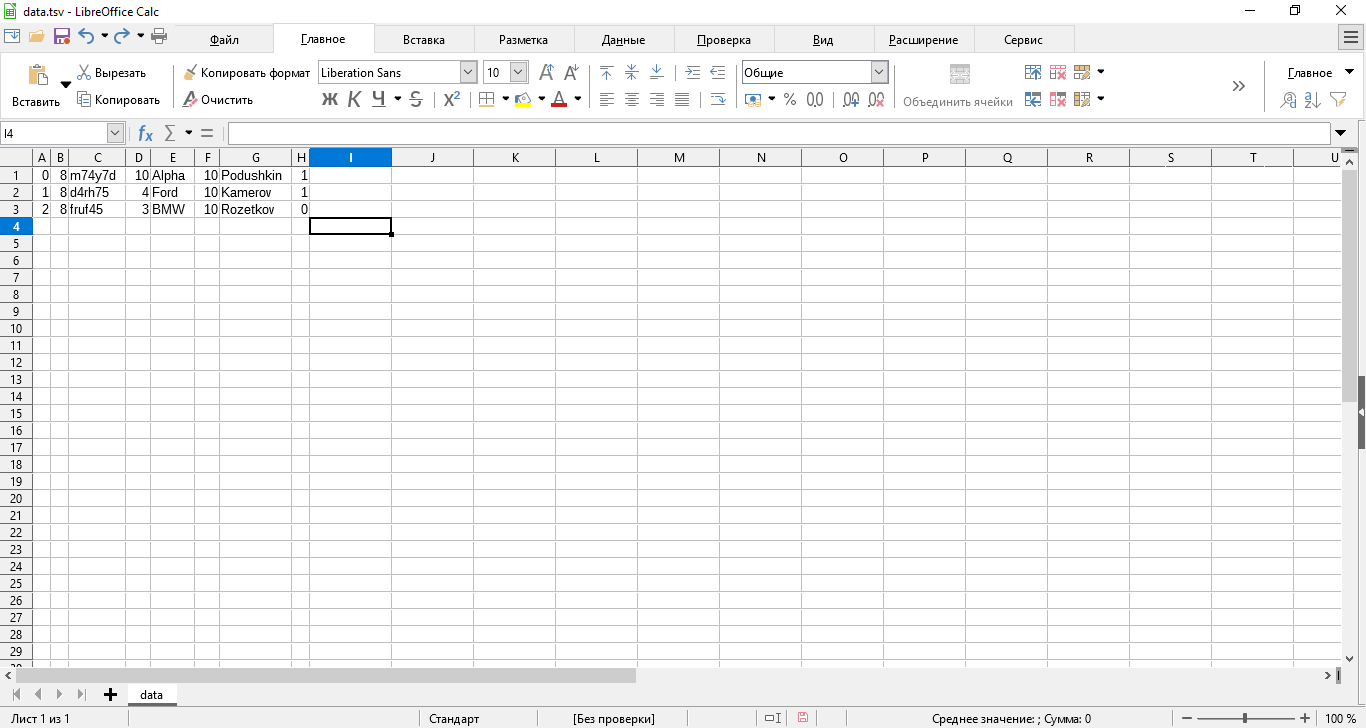
\includegraphics[width=16cm]{../pics/data-tsv-on-libre-office-calc.png}
    }
    \caption{data.tsv}
    \label{fig:data-tsv}
\end{figure}

\begin{figure}[h]
    \center{
        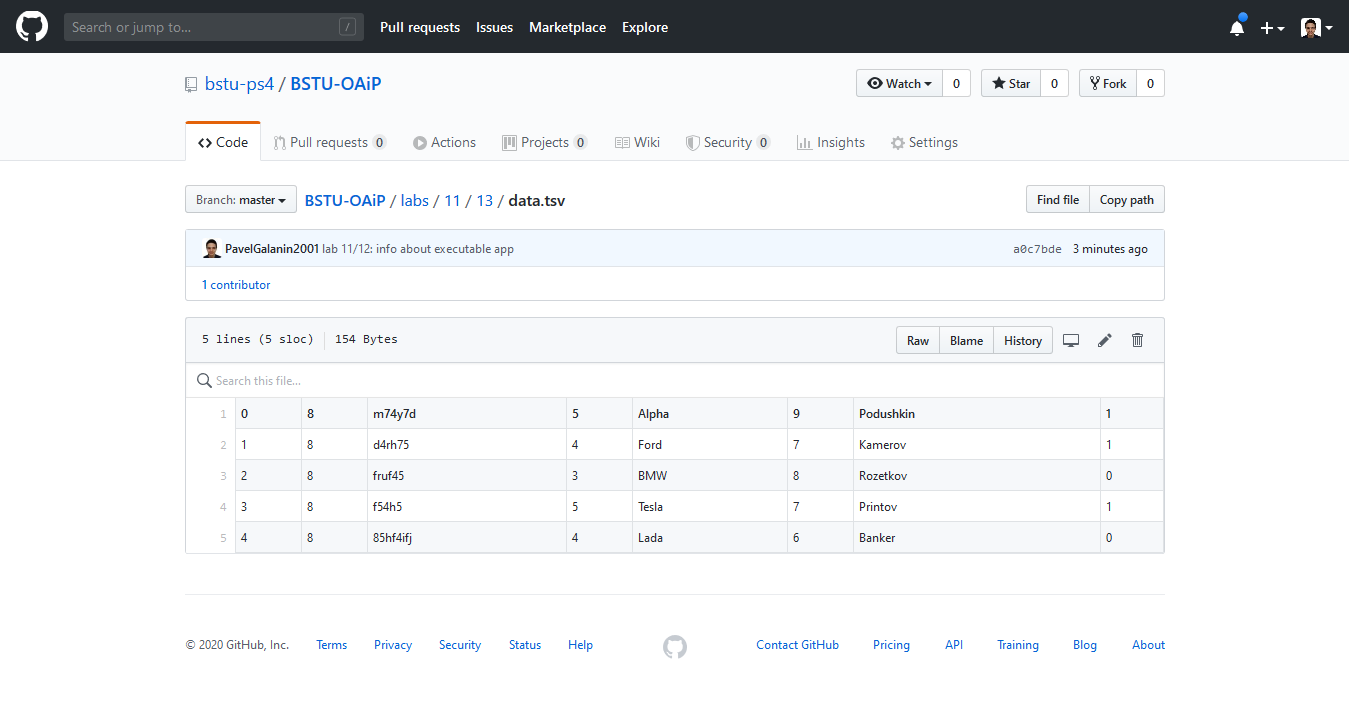
\includegraphics[width=16cm]{../pics/data-tsv-on-github.png}
    }
    \caption{data.tsv}
    \label{fig:data-tsv-on-github}
\end{figure}

% = = = = = Открытие файла

\subsubsection{Открытие файла}

Проредактировав поля в Libre Office Calc, файл содержит:

\begin{tcolorbox}
\begin{verbatim}
0	8	m74y7d	5	Alpha	9	Podushkin	1
1	8	d4rh75	4	Ford	7	Kamerov	1
2	8	fruf45	3	BMW	8	Rozetkov	0
3	8	f54h5	5	Tesla	7	Printov	1
4	8	85hf4ifj	4	Lada	6	Banker	0
\end{verbatim}
\end{tcolorbox}

Захожу в свою программу. Из меню выбираю пункт 1, чтобы открыть файл.

\begin{tcolorbox}
\begin{verbatim}
Размер пути файла: 
\end{verbatim}
\end{tcolorbox}

Ввожу размер пути файла.

\begin{tcolorbox}
\begin{verbatim}
Размер пути файла: 10
Какой файл открыть:     
\end{verbatim}
\end{tcolorbox}

Ввожу путь до файла. У меня это \textbf{data.tsv}. В консоли всякая информация, что файл сохранен в струтуру.

\begin{verbatim}
Размер пути файла: 10
Какой файл открыть: data.tsv
 = = = = = case 0 = = = = =
0
 = = = = = case 1 = = = = =
8
 = = = = = case 2 = = = = =
m74y7d
 = = = = = case 3 = = = = =
5
 = = = = = case 4 = = = = =
Alpha
 = = = = = case 5 = = = = =
9
 = = = = = case 6 = = = = =
Podushkin
 = = = = = case 7 = = = = =
1
 = = = = = case 0 = = = = =
1
 = = = = = case 1 = = = = =
8
 = = = = = case 2 = = = = =
d4rh75
 = = = = = case 3 = = = = =
4
 = = = = = case 4 = = = = =
Ford
 = = = = = case 5 = = = = =
7
 = = = = = case 6 = = = = =
Kamerov
 = = = = = case 7 = = = = =
1
 = = = = = case 0 = = = = =
2
 = = = = = case 1 = = = = =
8
 = = = = = case 2 = = = = =
fruf45
 = = = = = case 3 = = = = =
3
 = = = = = case 4 = = = = =
BMW
 = = = = = case 5 = = = = =
8
 = = = = = case 6 = = = = =
Rozetkov
 = = = = = case 7 = = = = =
0
 = = = = = case 0 = = = = =
3
 = = = = = case 1 = = = = =
8
 = = = = = case 2 = = = = =
f54h5
 = = = = = case 3 = = = = =
5
 = = = = = case 4 = = = = =
Tesla
 = = = = = case 5 = = = = =
7
 = = = = = case 6 = = = = =
Printov
 = = = = = case 7 = = = = =
1
 = = = = = case 0 = = = = =
4
 = = = = = case 1 = = = = =
8
 = = = = = case 2 = = = = =
85hf4ifj
 = = = = = case 3 = = = = =
4
 = = = = = case 4 = = = = =
Lada
 = = = = = case 5 = = = = =
6
 = = = = = case 6 = = = = =
Banker
 = = = = = case 7 = = = = =
0
Нажмите любую клавишу для продолжения...
\end{verbatim}

Нажимаю любую клавишу. В меню выбираю пунтк 3, чтобы вывести таблицу в консоль.

\begin{tcolorbox}
\begin{verbatim}
| ID   | байт Номер    | байт Марка    | байт Фамилия      | Осмотр     |
| ---- | ---- -------- | ---- -------- | ---- ------------ | ---------- |
| 0    | 8    m74y7d   | 5    Alpha    | 9    Podushkin    | Не пройден |
| 1    | 8    d4rh75   | 4    Ford     | 7    Kamerov      | Не пройден |
| 2    | 8    fruf45   | 3    BMW      | 8    Rozetkov     | Пройден    |
| 3    | 8    f54h5    | 5    Tesla    | 7    Printov      | Не пройден |
| 4    | 8    85hf4ifj | 4    Lada     | 6    Banker       | Пройден    |
Нажмите любую клавишу для продолжения...   
\end{verbatim}
\end{tcolorbox}

Структуры успешно обновилась.

\subsubsection{Если файл не найден}

Выбираю из меню пункт 1, чтобы открыть файл. Ввожу размер файла и не существующий путь

\begin{tcolorbox}
\begin{verbatim}
Размер пути файла: 10
Какой файл открыть: uirg
\end{verbatim}
\end{tcolorbox}

Появиться сообщение, что файл не найден. Также будет меню, чтобы выйти в главное меню, либо же остаться открывать файл.

\begin{tcolorbox}
\begin{verbatim}
Файл не найден!

Меню:
1. Открыть файл
0. Выйти в главное меню
\end{verbatim}
\end{tcolorbox}
